\documentclass[11pt,twoside,a4paper]{article}
\usepackage{comment}
\usepackage{url}
%
\usepackage[breaklinks]{hyperref}
\usepackage{breakurl}


\usepackage[ruled]{algorithm2e}



%\usepackage{lineno}
%\modulolinenumbers[5]

%\journal{Optics Communications}

%%%%%%%%%%%%%%%%%%%%%%%
%% Elsevier bibliography styles
%%%%%%%%%%%%%%%%%%%%%%%
%% To change the style, put a % in front of the second line of the current style and
%% remove the % from the second line of the style you would like to use.
%%%%%%%%%%%%%%%%%%%%%%%

%% Numbered
%\bibliographystyle{model1-num-names}

%% Numbered without titles
%\bibliographystyle{model1a-num-names}

%% Harvard
%\bibliographystyle{model2-names.bst}\biboptions{authoryear}

%% Vancouver numbered
%\usepackage{numcompress}\bibliographystyle{model3-num-names}

%% Vancouver name/year
%\usepackage{numcompress}\bibliographystyle{model4-names}\biboptions{authoryear}

%% APA style
%\bibliographystyle{model5-names}\biboptions{authoryear}

%% AMA style
%\usepackage{numcompress}\bibliographystyle{model6-num-names}

%% `Elsevier LaTeX' style
%\bibliographystyle{elsarticle-num}
%%%%%%%%%%%%%%%%%%%%%%%
\usepackage[]{graphicx}

%%%%%%%%%%%%%%%%%%%%%%%%%%%%%%%%%%%%%%%%%%%%%%%%%%%%%%%%%%%%%%%%%%%%%%%%%%%%%%%%%%

\usepackage[svgnames]{xcolor} % Enabling colors by their 'svgnames'

\usepackage{amsmath}
\usepackage{amsfonts}
\usepackage{amssymb}
\usepackage{blkarray}
%%%%%%%%%%%%%%%%%%%%%%%%%%%%%%%%%%%%%%%%%%%%%%%%%%%%%%%%%%%%%%%%%%%%%%%%%%%%%%%%%%

\newcommand{\MATRIX}[1]{\mathbf{\uppercase{#1}}}
\newcommand{\VECTOR}[1]{\mathbf{\lowercase{#1}}}


%% diagonal function
\newcommand{\funcdiag}{diag}


%%%%%%%%%%%%%%%%%%%%%%%%%%%%%%%%%%%%%%%%%%%%%%%%%%%%%%%%%%%%%%%%%%%%%%%%%%%%%%%%%%
\usepackage{titlesec}
\titleformat{\section}
  {\normalfont\Large\bfseries}{\thesection}{1em}{}[{\titlerule[0.8pt]}]

\titleformat{\subsection}
  {\normalfont\Large\bfseries}{\thesubsection}{1em}{}[]

%%%%%%%%%%%%%%%%%%%%%%%%%%%%%%%%%%%%%%%%%%%%%%%%%%%%%%%%%%%%%%%%%%%%%%%%%%%%%%%%%%
%%%%%%%%%%%%%%%%%%%%%%%%%%%%%%%%%%%%%%%%%%%%%%%%%%%%%%%%%%%%%%%%%%%%%%%%%%%%%%%%%%
\usepackage[a4paper,bindingoffset=0.5cm,%
            left=2.5cm,right=2.5cm,top=2.5cm,bottom=2.5cm,%
            footskip=0.625cm]{geometry}


%%%%%%%%%%%%%%%%%%%%%%%%%%%%%%%%%%%%%%%%%%%%%%%%%%%%%%%%%%%%%%%%%%%%%%%%%%%%%%%%%%
%%%%%%%%%%%%%%%%%%%%%%%%%%%%%%%%%%%%%%%%%%%%%%%%%%%%%%%%%%%%%%%%%%%%%%%%%%%%%%%%%%
\begin{document} 
\title{Relation Between the Mass-Spring System and the Dynamic Speckle}
%\tnotetext[mytitlenote]{Fully documented templates are available in the 
%elsarticle package on \href{http://www.ctan.org/tex-archive/macros/latex/contrib/elsarticle}{CTAN}.}

% Group authors per affiliation:
\author{-------- ------- ------}
\author{-------- ------- ------}

% \author{Fernando Pujaico Rivera\fnref{myfootnote2}}
% \author{Roberto Alves Braga Jr.\fnref{myfootnote1}}
% \address{University Federal of Lavras, Lavras, Brazil}
% \fntext[myfootnote2]{201518201@posgrad.ufla.br}
% \fntext[myfootnote1]{robertobraga@deg.ufla.br }

%\begin{abstract}
%In this article will be studied the relation between the mass-spring system and the dynamic speckle.
%\end{abstract}

%\begin{keyword}
%Biospeckle laser \sep 
%Biospeckle signal\sep 
%Dynamic speckle \sep  
%\end{keyword}

\maketitle
%%%%%%%%%%%%%%%%%%%%%%%%%%%%%%%%%%%%%%%%%%%%%%%%%%%%%%%%%%%%%%%%%%%%%%%%%%%%%%%%%%%%%%%%%
%%%%%%%%%%%%%%%%%%%%%%%%%%%%%%%%%%%%%%%%%%%%%%%%%%%%%%%%%%%%%%%%%%%%%%%%%%%%%%%%%%%%%%%%%
\section{Introduction}
The biospeckle laser analysis has presented as a versatile tool in the analysis of
biological activity. 

%%%%%%%%%%%%%%%%%%%%%%%%%%%%%%%%%%%%%%%%%%%%%%%%%%%%%%%%%%%%%%%%%%%%%%%%%%%%%%%%%%%%%%%%%
%%%%%%%%%%%%%%%%%%%%%%%%%%%%%%%%%%%%%%%%%%%%%%%%%%%%%%%%%%%%%%%%%%%%%%%%%%%%%%%%%%%%%%%%%
\section{System description}
The signal $y$ with samples $y(n)$, 
represent the adquisition of the signal $x_M$ with samples $x_{M}(n)$, 
obtained  in a mass-spring system of $M$ elements, where each mass
is separated of another by a distance of $L/M$, like can be seen in the
Fig. \ref{fig:system}.
\begin{figure}[ht!]
\centering
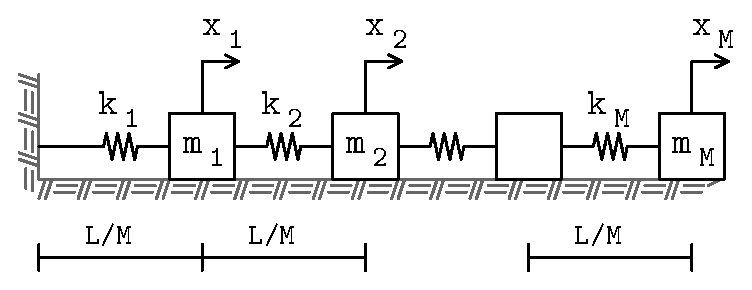
\includegraphics[width=0.95\columnwidth]{images/system-mass-spring.eps}
\caption{Data acquisition system setup of the coffee seed.  }
\label{fig:system}
\end{figure}

Thus, in this system the mass are denoted as $m_i$, the springs as $k_i$ and the
displacements of each mass by $x_i$, for all $1 \leq  i\leq M$.

The objective of this work it is to solve the next inverse problem: Known $y(n)$, 
and assuming $M$ elements with $m_i=m=1/L$; 
what values of $k_i$ generate a signal $x_M$ that minimize $E$, 
where
\begin{equation}\label{eq:inverseproblem}
 E=\frac{1}{2}\sum_{n} (y(n)-x_M(n))^2
\end{equation} 

%%%%%%%%%%%%%%%%%%%%%%%%%%%%%%%%%%%%%%%%%%%%%%%%%%%%%%%%%%%%%%%%%%%%%%%%%%%%%%%%%%%%%%%%%
%%%%%%%%%%%%%%%%%%%%%%%%%%%%%%%%%%%%%%%%%%%%%%%%%%%%%%%%%%%%%%%%%%%%%%%%%%%%%%%%%%%%%%%%%
\section{Mass-spring system}
Assuming a mass spring system like seen in the Fig. \ref{fig:system} with $m_i=m$
we can to get the system of Eq. (\ref{eq:massspring1}).

\begin{equation}\label{eq:massspring1}
 m \VECTOR{\ddot{X}} = -\MATRIX{P} \VECTOR{X},
\end{equation}
where
\begin{equation}\label{eq:X}
 \VECTOR{X} = \left( 
 \begin{matrix}
 x_1\\
 x_2\\ 
 x_3\\ 
 \vdots \\
 x_{N-1}\\
 x_N\\
 \end{matrix}
\right)
\end{equation}
and 
\begin{equation}\label{eq:P}
 \MATRIX{P}(\VECTOR{k}) \equiv \MATRIX{P} = \left( 
 \begin{matrix}
 k_1+k_2 & -k_2    & 0       &  \hdots & 0           & 0  \\
 -k_2    & k_2+k_3 & -k_3    &  \hdots & 0           & 0  \\
 0       &    -k_3 & k_3+k_4 &  \hdots & 0           & 0  \\
 \vdots  & \vdots  & \vdots  &  \ddots & \vdots      & \vdots \\
 0       & 0       & 0       &  \hdots & x_{N-1}+x_N & -x_N  \\
 0       & 0       & 0       &  \hdots & -x_N        & x_N  \\
 \end{matrix}
\right),
\end{equation}
so that $\MATRIX{P}$ is a function of $\VECTOR{k}=( k_1~ k_2~ k_3~ \hdots ~ k_{M-1}~ k_M)^{T}$.


%%%%%%%%%%%%%%%%%%%%%%%%%%%%%%%%%%%%%%%%%%%%%%%%%%%%%%%%%%%%%%%%%%%%%%%%%%%%%%%%%%%%%%%%%
\subsection{Exact solution}
Knowing the system shown in the Eq. (\ref{eq:massspring1}), we can solve It
using the Eq. (\ref{eq:Xt}),
\begin{equation}\label{eq:Xt}
 \VECTOR{X}(t)= \MATRIX{V}\left(\MATRIX{D}_1 cos(\mathbf{w}t) + \MATRIX{D}_2 sin(\mathbf{w}t) \right),
\end{equation}
or Eq. (\ref{eq:Xtalt})
\begin{equation}\label{eq:Xtalt}
 \VECTOR{X}(t)= \MATRIX{V}\left( \funcdiag(cos(\VECTOR{w}t))\VECTOR{d}_1 +  \funcdiag(sin(\VECTOR{w}t))\VECTOR{d}_2 \right),
\end{equation}
where, $\MATRIX{V}=\left(\VECTOR{e}_1,\VECTOR{e}_2, ..., \VECTOR{e}_M \right)$ and 
$\mathbf{w}=\left( \sqrt{\lambda_1},\sqrt{\lambda_2},\dots ,\sqrt{\lambda_M}\right)^{T}$ 
are a matrix and a column 
vector conform using the eigenvectors $\VECTOR{e}_i$ and eigenvalues $\lambda_i$ of
$\MATRIX{P}/m$.
By other side, $\MATRIX{D}_1$ and $\MATRIX{D}_2$ are two any constant diagonal matrices
conform by the elements of column vectors $\VECTOR{d}_1$ and $\VECTOR{d}_2$ respectively.
Thus, we now that $\dot{\VECTOR{X}}(t)$ and $\ddot{\VECTOR{X}}(t)$ are defined by the Eqs. (\ref{eq:dXt_dt})
and (\ref{eq:d2Xt_dt2}) respectively.
\begin{equation}\label{eq:dXt_dt}
 \dot{\VECTOR{X}}(t)= \MATRIX{V}\left(-\MATRIX{D}_1 \MATRIX{W} sin(\mathbf{w}t)) + \MATRIX{D}_2 \MATRIX{W} cos(\mathbf{w}t) \right),
\end{equation}
\begin{equation}\label{eq:d2Xt_dt2}
 \ddot{\VECTOR{X}}(t)= -\MATRIX{V}\left(\MATRIX{D}_1 \MATRIX{W}^2 cos(\mathbf{w}t) + \MATRIX{D}_2 \MATRIX{W}^2 sin(\mathbf{w}t) \right),
\end{equation}
being $\MATRIX{W}$ a diagonal matrix conform with the elements of vector $\mathbf{w}$;
thus, It is fulfill that $\MATRIX{W}^2=(\MATRIX{V} \MATRIX{D}_1)^{-1}(\MATRIX{P}/m)(\MATRIX{V} \MATRIX{D}_1)=(\MATRIX{V} \MATRIX{D}_2)^{-1}(\MATRIX{P}/m)( \MATRIX{V} \MATRIX{D}_2)$.

\subsubsection{Constant values from two points}
Now, to get the constant values in the column vectors $\VECTOR{d}_1$ and $\VECTOR{d}_2$, we can
use the Eq. (\ref{eq:d1d2})
\begin{equation}\label{eq:d1d2}
  \left( 
 \begin{matrix}
\MATRIX{V}\funcdiag(cos(\VECTOR{w}t_1) & \MATRIX{V}\funcdiag(sin(\VECTOR{w}t_1))\\
\MATRIX{V}\funcdiag(cos(\VECTOR{w}t_2)) & \MATRIX{V}\funcdiag(sin(\VECTOR{w}t_2))\\
 \end{matrix}
 \right)^{-1}
 \left( 
 \begin{matrix}
\VECTOR{X}(t_1) \\
\VECTOR{X}(t_2)
 \end{matrix}
 \right)=
  \left( 
 \begin{matrix}
\VECTOR{d}_1 \\
\VECTOR{d}_2
 \end{matrix}
 \right)
\end{equation}

\subsubsection{Constant values from position and velocity of a point}
Now, to get the constant values in the column vectors $\VECTOR{d}_1$ and $\VECTOR{d}_2$, we can
use the Eq. (\ref{eq:d1d22})
\begin{equation}\label{eq:d1d22}
  \left( 
 \begin{matrix}
\MATRIX{V}\funcdiag(cos(\VECTOR{w}t_1)) & \MATRIX{V}\funcdiag(sin(\VECTOR{w}t_1))\\
-\MATRIX{V}\MATRIX{W}\funcdiag(sin(\VECTOR{w}t_1)) & \MATRIX{V}\MATRIX{W}\funcdiag(cos(\VECTOR{w}t_1))\\
 \end{matrix}
 \right)^{-1}
 \left( 
 \begin{matrix}
\VECTOR{X}(t_1) \\
\dot{\VECTOR{X}}(t_1)
 \end{matrix}
 \right)=
  \left( 
 \begin{matrix}
\VECTOR{d}_1 \\
\VECTOR{d}_2
 \end{matrix}
 \right)
\end{equation}

%%%%%%%%%%%%%%%%%%%%%%%%%%%%%%%%%%%%%%%%%%%%%%%%%%%%%%%%%%%%%%%%%%%%%%%%%%%%%%%%%%%%%%%%%
\subsection{Finite differences: Knowing two consecutive samples}
\label{subsec:findiff1}
Applying finite differences we known that $\VECTOR{X} \equiv \VECTOR{X}(n)$ and
$\VECTOR{\ddot{X}} \equiv$ $( \VECTOR{X}(n+1)$ $-2\VECTOR{X}(n)$ $+\VECTOR{X}(n-1) ) /{\tau^2}$,
so that the Eq. (\ref{eq:massspring1}) can be rewrite as
\begin{equation}\label{eq:massspring2}
 \VECTOR{X}(n) = \left(2 \mathbf{I} -\MATRIX{P}\frac{\tau^2}{m}\right) \VECTOR{X}(n-1)-\VECTOR{X}(n-2),
\end{equation}
now deriving $\VECTOR{X}(n)$ by the vector $\VECTOR{k}=( k_1~ k_2~ k_3~ \hdots ~ k_{M-1}~ k_M)$,
so that $\MATRIX{J}(n) \equiv \frac{\partial \VECTOR{X}(n)}{\partial \VECTOR{k}}$,
we get the Eq.  (\ref{eq:massspring3})
\begin{equation}\label{eq:massspring3}
 \MATRIX{J}(n) = 
 -\frac{\tau^2}{m}\bigcup_{i}{ \left[ \frac{ \partial \MATRIX{P} }{\partial k_{i}}  \VECTOR{X}(n-1)\right] }
 +\left(2 \mathbf{I} -\MATRIX{P}\frac{\tau^2}{m}\right) \MATRIX{J}(n-1)
 -\MATRIX{J}(n-2),
\end{equation}
where 
\begin{equation}\label{eq:dPdki}
 \frac{ \partial \MATRIX{P}}{\partial k_{i}} = 
 \begin{blockarray}{cccccccc}
 ~       &  ~       & ~       & i-th    & ~       & ~           & ~  & ~\\
 \begin{block}{(ccccccc)c}
 0       &  \hdots & 0       & 0       &  \hdots & 0           & 0  & ~\\
 \vdots  &  \hdots & \vdots  & \vdots  &  \hdots & \vdots      & \vdots & ~\\
 0       &  \hdots & 1       & -1      &  \hdots & 0           & 0  & ~\\
 0       &  \hdots & -1      & 1       &  \hdots & 0           & 0  & i-th\\
 \vdots  &  \hdots & \vdots  & \vdots  &  \ddots & \vdots      & \vdots & ~\\
 0       &  \hdots & 0       & 0       &  \hdots & 0           & 0  & ~\\
 0       &  \hdots & 0       & 0       &  \hdots & 0           & 0  & ~\\
\end{block}
\end{blockarray}
,
\end{equation}


%%%%%%%%%%%%%%%%%%%%%%%%%%%%%%%%%%%%%%%%%%%%%%%%%%%%%%%%%%%%%%%%%%%%%%%%%%%%%%%%%%%%%%%%%
\subsection{Finite differences: Knowing one sample and velocity}
In this case, It is necessary define $\VECTOR{\dot{X}} = \VECTOR{V}$, so that
the Eq. (\ref{eq:massspring1}) can be rewrite as
\begin{equation}\label{eq:massspringm2}
\left(
\begin{matrix}
 \VECTOR{\dot{X}}\\
 \VECTOR{\dot{V}}\\
\end{matrix}\right)=
\left(
\begin{matrix}
 \mathbf{0}    & \MATRIX{I}_{M \times M} \\
 -\MATRIX{P}/m & \mathbf{0} \\
\end{matrix}\right)
\left(
\begin{matrix}
 \VECTOR{X}\\
 \VECTOR{V}\\
\end{matrix}\right),
\end{equation}
so that we got
\begin{equation}\label{eq:massspringm2a}
 \VECTOR{\dot{U}}=A\VECTOR{U},
\end{equation}
where $\VECTOR{U}= \left( \VECTOR{X} ; \VECTOR{V} \right)$ and
$A=\left( \mathbf{0} , \MATRIX{I}_{M \times M} ; -\MATRIX{P}/m , \mathbf{0} \right)$.

Applying finite differences we known that $\VECTOR{U} \equiv \VECTOR{U}(n)$ and
$\VECTOR{\dot{U}} \equiv$ $( \VECTOR{U}(n)$ $-\VECTOR{U}(n-1)$ $ ) /{\tau_2}$, 
so that the Eq. (\ref{eq:massspringm2a}) can be rewrite as
\begin{equation}\label{eq:massspring2m2}
 \VECTOR{U}(n) = \left( \mathbf{I} -\mathbf{A}\tau_2 \right)^{-1} \VECTOR{U}(n-1),
\end{equation}
\textcolor{red}{Problems  with finite differences: To got a good aproximation it 
is necessary to choose $\tau_2 \gg \tau$ (where $\tau$ is the value used in the section \ref{subsec:findiff1}). Experimentaly was see that $\tau_2 \geq \tau^2$.}

Now deriving $\VECTOR{U}(n)$ by the vector $\VECTOR{k}=( k_1~ k_2~ k_3~ \hdots ~ k_{M-1}~ k_M)$,
so that $\MATRIX{Q}(n) \equiv \frac{\partial \VECTOR{U}(n)}{\partial \VECTOR{k}}$,
we get the Eq.  (\ref{eq:massspring3m2})
\begin{equation}\label{eq:massspring3m2}
 \MATRIX{Q}(n) = 
  \tau_2 \left( \mathbf{I} -\mathbf{A}\tau_2 \right)^{-1} \bigcup_{i}{ \left[ \frac{ \partial \mathbf{A} }{\partial k_{i}}  \VECTOR{U}(n)\right] },
 +\left( \mathbf{I} -\mathbf{A}\tau_2 \right)^{-1} \MATRIX{Q}(n-1),
\end{equation}
where 
\begin{equation}\label{eq:dPdkim2}
 \frac{ \partial \mathbf{A} }{\partial k_{i}} = 
\left(
\begin{matrix}
 \mathbf{0}    & \mathbf{0}_{M \times M} \\
 -\frac{1}{m}\frac{ \partial\MATRIX{P}}{\partial k_{i}} & \mathbf{0} \\
\end{matrix}\right)
,

\end{equation}
%%%%%%%%%%%%%%%%%%%%%%%%%%%%%%%%%%%%%%%%%%%%%%%%%%%%%%%%%%%%%%%%%%%%%%%%%%%%%%%%%%%%%%%%%
%%%%%%%%%%%%%%%%%%%%%%%%%%%%%%%%%%%%%%%%%%%%%%%%%%%%%%%%%%%%%%%%%%%%%%%%%%%%%%%%%%%%%%%%%
\section{Minimization problem}
The minimization problem seen in the Eq. (\ref{eq:inverseproblem}) can be rewrite as
\begin{equation}\label{eq:minimization1}
 E(\VECTOR{k})=\frac{1}{2}\sum_{n} \left( y(n)-\VECTOR{b}^{T}\VECTOR{X}(n,\VECTOR{k}) \right)^2
\end{equation}
where $\VECTOR{b}=( 0~ 0~ 0~ \hdots ~ 0~ 1)^{T}$, $y(n)$ are known values and 
$\VECTOR{X}(n)$ that is a function of $\VECTOR{k}=( k_1~ k_2~ k_3~ \hdots ~ k_{M-1}~ k_M)^{T}$.

Now, knowing that a minimum of $E(\VECTOR{k})$ in $\VECTOR{k}$ is found when 
$\frac{\partial E(\VECTOR{k})}{\partial k_i}=0$ for all integer $1 \leq i \leq M$; we calculate the
Eq. (\ref{eq:minimization1d}).
\begin{equation}\label{eq:minimization1d}
 \frac{\partial E(\VECTOR{k})}{\partial k_i}=\sum_{n}{\left( \VECTOR{b}^{T}\frac{\partial \VECTOR{X}(n,\VECTOR{k})}{\partial k_i}\right)^{T} \left( \VECTOR{b}^{T}\VECTOR{X}(n,\VECTOR{k}) -y(n)  \right) },
\end{equation}

Now reordering the Eq. 
(\ref{eq:minimization1d}) using a vectorial differentiation by $\VECTOR{k}$, we get the 
Eq. (\ref{eq:minimization2}).
\begin{equation}\label{eq:minimization2}
 \frac{\partial E(\VECTOR{k})}{\partial \VECTOR{k}}=\sum_{n}{ \left( \VECTOR{b}^{T}\MATRIX{J}(n,\VECTOR{k})\right)^{T} \left(\VECTOR{b}^{T}\VECTOR{X}(n,\VECTOR{k}) -y(n) \right) },
\end{equation}

where $\MATRIX{J}(n)=\frac{\partial \VECTOR{X}(n)}{\partial \VECTOR{k}}$.

%%%%%%%%%%%%%%%%%%%%%%%%%%%%%%%%%%%%%%%%%%%%%%%%%%%%%%%%%%%%%%%%%%%%%%%%%%%%%%%%%%%%%%%%%
\subsection{Landweber iterative method}
The Landweber iteration method propose that 
the minimization of a nonlinear function $E(\VECTOR{k})$ can be found using
the gradient descent method, so that 

\begin{equation}\label{eq:Landweber1}
\VECTOR{k}_{j}\leftarrow \VECTOR{k}_{j-1} - \alpha \frac{\partial E(\VECTOR{k}_{j-1})}{\partial \VECTOR{k}}
\end{equation}
where $0 < \alpha < 2/||\frac{\partial E(\VECTOR{k})}{\partial \VECTOR{k}}||^2$ and
$\|\cdot \|$ is the spectral norm. Thus, following the Landweber iteration method
and using the Eq. (\ref{eq:minimization2}) in
our minimization problem, It can be solved using the Eq. (\ref{eq:Landweber2}).
\begin{equation}\label{eq:Landweber2}
\VECTOR{k}_{j}\leftarrow \VECTOR{k}_{j-1} 
- \alpha \sum_{n}{ \left( \VECTOR{b}^{T}\MATRIX{J}(n,\VECTOR{k}_{j-1})\right)^{T} \left(\VECTOR{b}^{T}\VECTOR{X}(n,\VECTOR{k}_{j-1}) -y(n) \right) }
\end{equation}
%%%%%%%%%%%%%%%%%%%%%%%%%%%%%%%%%%%%%%%%%%%%%%%%%%%%%%%%%%%%%%%%%%%%%%%%%%%%%%%%%%%%%%%%%
\subsection{Tikhonov iterative method}

If we assume that the problem of to get $\VECTOR{k}$ will be solved iteratively, 
we can  rewrite the Eq. (\ref{eq:minimization2}) as if was evaluated by $\VECTOR{X}_{j}(n)$
and $\MATRIX{J}_{j-1}(n)$, as in the Eq. (\ref{eq:miniterative}).
\begin{equation}\label{eq:miniterative}
\sum_{n}{\left\{ \left( \VECTOR{b}^{T}\MATRIX{J}_{j-1}(n)\right)^{T} \left(\VECTOR{b}^{T}\VECTOR{X}_{j}(n) - y(n)  \right) \right \}}=\mathbf{0}.
\end{equation}
Where $\MATRIX{J}_{j-1}(n)=\MATRIX{J}(n,\VECTOR{k}_{j-1})$ and
$\VECTOR{X}_{j}(n)=\VECTOR{X}(n,\VECTOR{k}_{j-1})$.

Knowing by the Taylor theorem that 
$\VECTOR{X}_{j}(n) \approx \VECTOR{X}_{j-1}(n) + \MATRIX{J}_{j-1}(n)\left( \VECTOR{k}_{j} - \VECTOR{k}_{j-1}\right) $

\begin{equation}\label{eq:miniterative2}
\VECTOR{k}_{j} = \VECTOR{k}_{j-1} +
\left(\sum_{n}{ \left( \VECTOR{b}^{T}\MATRIX{J}_{j-1}(n)\right)^{T}\left(  \VECTOR{b}^{T}\MATRIX{J}_{j-1}(n) \right) }\right)^{-1} 
\sum_{n}{ \left( \VECTOR{b}^{T}\MATRIX{J}_{j-1}(n)\right)^{T} \left(y(n) - \VECTOR{b}^{T}\VECTOR{X}_{j-1}(n) \right) }.
\end{equation}

joint with the Eqs. (\ref{eq:massspring2}) and (\ref{eq:massspring3}) we got:
\begin{equation}\label{eq:massspring2b}
 \VECTOR{X}(n,\VECTOR{k}) = \left(2 \mathbf{I} -\mathbf{P(\VECTOR{k})}\frac{\tau^2}{m}\right) \VECTOR{X}(n-1,\VECTOR{k})-\VECTOR{X}(n-2,\VECTOR{k}),
\end{equation}

\begin{equation}\label{eq:massspring3b}
 \MATRIX{J}(n,\VECTOR{k}) = 
 -\frac{\tau_2^2}{m}\bigcup_{i}{ \left[ \frac{ \partial\left(\MATRIX{P}\right)}{\partial k_{i}}  \VECTOR{X}(n-1,\VECTOR{k})\right] }
 +\left(2 \mathbf{I} -\mathbf{P(\VECTOR{k})}\frac{\tau_2^2}{m}\right) \MATRIX{J}(n-1,\VECTOR{k})
 -\MATRIX{J}(n-2,\VECTOR{k}),
\end{equation}
%%%%%%%%%%%%%%%%%%%%%%%%%%%%%%%%%%%%%%%%%%%%%%%%%%%%%%%%%%%%%%%%%%%%%%%%%%%%%%%%%%%%%%%%%
%%%%%%%%%%%%%%%%%%%%%%%%%%%%%%%%%%%%%%%%%%%%%%%%%%%%%%%%%%%%%%%%%%%%%%%%%%%%%%%%%%%%%%%%%
\section{Numerical results} 
\label{sec:numerical}
oioio


%%%%%%%%%%%%%%%%%%%%%%%%%%%%%%%%%%%%%%%%%%%%%%%%%%%%%%%%%%%%%%%%%%%%%%%%%%%%%%%%%%%%%%%%%
%%%%%%%%%%%%%%%%%%%%%%%%%%%%%%%%%%%%%%%%%%%%%%%%%%%%%%%%%%%%%%%%%%%%%%%%%%%%%%%%%%%%%%%%%
\section{Conclusion} 

In this work were presented

\section{Acknowledgment}
We wish to acknowledge the partial financial support for this study provided by the $CAPES$ 
scholarship
$PNPD$ Program, $FAPEMIG$ and $CNPQ$.

%----------------------------------------------------------------------------------------
%	REFERENCE LIST
%----------------------------------------------------------------------------------------
\section{Bibliography}
\bibliography{report}   %>>>> bibliography data in report.bib
\bibliographystyle{spiebib}   %>>>> makes bibtex use spiebib.bst


%----------------------------------------------------------------------------------------

\end{document} 
